\documentclass[a4paper]{article}
\usepackage[T1]{fontenc}			% pacchetto per \chapter
\usepackage[italian]{babel}
\usepackage[italian]{isodate}  		% formato delle date in italiano
\usepackage{graphicx}				% gestione delle immagini
\usepackage{amsfonts}
\usepackage{booktabs}				% tabelle di qualità superiore
\usepackage{mathrsfs, amsmath}				% pacchetto matematica
\usepackage{mathtools}				% per sottolineare sotto le equazioni
\usepackage{stmaryrd} 				% per '\llbracket' e '\rrbracket'
\usepackage{amsthm}					% teoremi migliorati
\usepackage{enumitem}				% gestione delle liste
\usepackage{pifont}					% pacchetto con elenchi carini
\usepackage{enumitem}				% pacchetto per elenchi con lettere dell'alfabeto
\usepackage{cancel}					% per cancellare delle espressioni matematiche
\usepackage{listings}				% implementa codice di programmazione
\usepackage{mathalpha}
\usepackage{caption}


\usepackage[x11names]{xcolor}		% pacchetto colori RGB
% Link ipertestuali per l'indice
\usepackage{xcolor}
\usepackage[linkcolor=black, citecolor=blue, urlcolor=cyan]{hyperref}
\hypersetup{
	colorlinks=true
}

% Colour code style
\definecolor{codegreen}{rgb}{0,0.6,0}
\definecolor{codegray}{rgb}{0.5,0.5,0.5}
\definecolor{codepurple}{rgb}{0.58,0,0.82}
\definecolor{backcolour}{rgb}{0.95,0.95,0.92}

\lstdefinestyle{MATLAB}{
	backgroundcolor=\color{backcolour},   
	commentstyle=\color{codegreen},
	keywordstyle=\color{magenta},
	numberstyle=\tiny\color{codegray},
	stringstyle=\color{codepurple},
	basicstyle=\ttfamily\footnotesize,
	breakatwhitespace=false,         
	breaklines=true,                 
	captionpos=b,                    
	keepspaces=true,                 
	numbers=left,                    
	numbersep=5pt,                  
	showspaces=false,                
	showstringspaces=false,
	showtabs=false,                  
	tabsize=2
}
\lstset{style=MATLAB}

%\usepackage{showframe}				% visualizzazione bordi
%\usepackage{showkeys}				% visualizzazione etichetta

\newtheorem{theorem}{\textcolor{Red3}{\underline{Teorema}}}
\newtheorem{lemma}{Lemma}
\renewcommand{\qedsymbol}{QED}
\newcommand{\exec}[1]{\llbracket #1\:\rrbracket}
\newcommand{\dquotes}[1]{``#1''}
\newcommand{\longline}{\noindent\rule{\textwidth}{0.4pt}}

\begin{document}
	\author{Università degli Studi di Verona}
	\title{Soluzione - Esame di Elaborazione di segnali e immagini}
	\date{{\Large 01 Febbraio 2023}}
	\maketitle
	
	\section{Soluzione Esercizio (10 punti)}
	\subsection*{Fonte: Simulazione 22/01/2020}
	
	Si rappresenta il segnale $G\left(\mu\right)$ nel dominio delle frequenze:
	\begin{equation*}
		G\left(\mu\right) = \underbrace{\Pi\left(\dfrac{\mu}{10}\right)}_{a} + \underbrace{2\Pi\left(\dfrac{\mu - 45}{30}\right)}_{b} + \underbrace{2\Pi\left(\dfrac{\mu + 45}{30}\right)}_{c}
	\end{equation*}
	Le lettere rappresentano:
	\begin{enumerate}[label=\alph*)]
		\item Una box larga $10$ centrata rispetto l'asse $y$ e alta $1$;
		\item Una box larga $30$ traslata a destra di $45$ e alta $2$;
		\item Una box larga $30$ traslata a sinistra di $45$ e alta $2$.
	\end{enumerate}
	Per descrivere il dominio duale si utilizzano le seguenti proprietà, con $x_{1}$ ed $x_{2}$ appartenenti ai due domini duali, rispettivamente:
	\begin{itemize}
		\item \textbf{Proprietà notevole}:
		\begin{equation*}
			\Pi\left(x_{1}\right) \xrightarrow{\mathscr{F}\left(\text{oppure } \mathscr{F}^{-1}\right)} \mathrm{sinc}\left(x_{2}\right)
		\end{equation*}
		
		\item \textbf{Proprietà di amplificazione}:
		\begin{equation*}
			A \: f\left(x_{1}\right) \xrightarrow{\mathscr{F}\left(\text{oppure } \mathscr{F}^{-1}\right)} A \: F\left(x_{2}\right)
		\end{equation*}
		
		\item \textbf{Scalatura temporale}:
		\begin{equation*}
			f\left(\dfrac{x_{1}}{b}\right) \xrightarrow{\mathscr{F}\left(\text{oppure } \mathscr{F}^{-1}\right)} b \cdot F\left(x_{2} \cdot b\right)
		\end{equation*}
		
		\item \textbf{Proprietà di shift nel tempo}:
		\begin{equation*}
			F\left(\mu - \mu_{0}\right) = f\left(t\right) \cdot e^{j2\pi t \mu_{0}}
		\end{equation*}
	\end{itemize}\newpage
	Il segnale nel dominio continuo del tempo:
	\begin{gather*}
		\begin{array}{lll}
			g\left(t\right) & = & 10\mathrm{sinc}\left(10t\right) + 2 \cdot 30\mathrm{sinc}\left(30t\right) \cdot e^{j 2 \pi t 45} + 2 \cdot 30\mathrm{sinc}\left(30t\right) \cdot e^{-j 2 \pi t 45} \\
			&& \\
							& = & 10\mathrm{sinc}\left(10t\right) + 60\mathrm{sinc}\left(30t\right) \cdot \left(e^{j 2 \pi t 45} + e^{-j 2 \pi t 45}\right) \\
			&& \\
							& = & 10\mathrm{sinc}\left(10t\right) + 60\mathrm{sinc}\left(30t\right) \cdot 2\cos\left(2\pi 45 t\right)
		\end{array}\\
		\text{dato che } \cos\left(\theta\right) = \dfrac{e^{j\theta} + e^{-j \theta}}{2}
	\end{gather*}
	Adesso si eseguono le elaborazioni a cui è sottoposto il segnale $g\left(t\right)$. La prima operazione da applicare è il \textbf{passo basso ideale} con frequenza di taglio $10$ Hz:
	\begin{equation*}
		\begin{array}{lll}
			\text{Dominio del tempo } & \longrightarrow & a\left(t\right) = g\left(t\right) * 20\mathrm{sinc}\left(20t\right) \\
			&& \\
			\text{Dominio delle frequenze } & \longrightarrow & A\left(\mu\right) = G\left(\mu\right) \cdot \Pi\left(\dfrac{\mu}{20}\right)
		\end{array}
	\end{equation*}
	\begin{figure}[!htp]
		\centering
		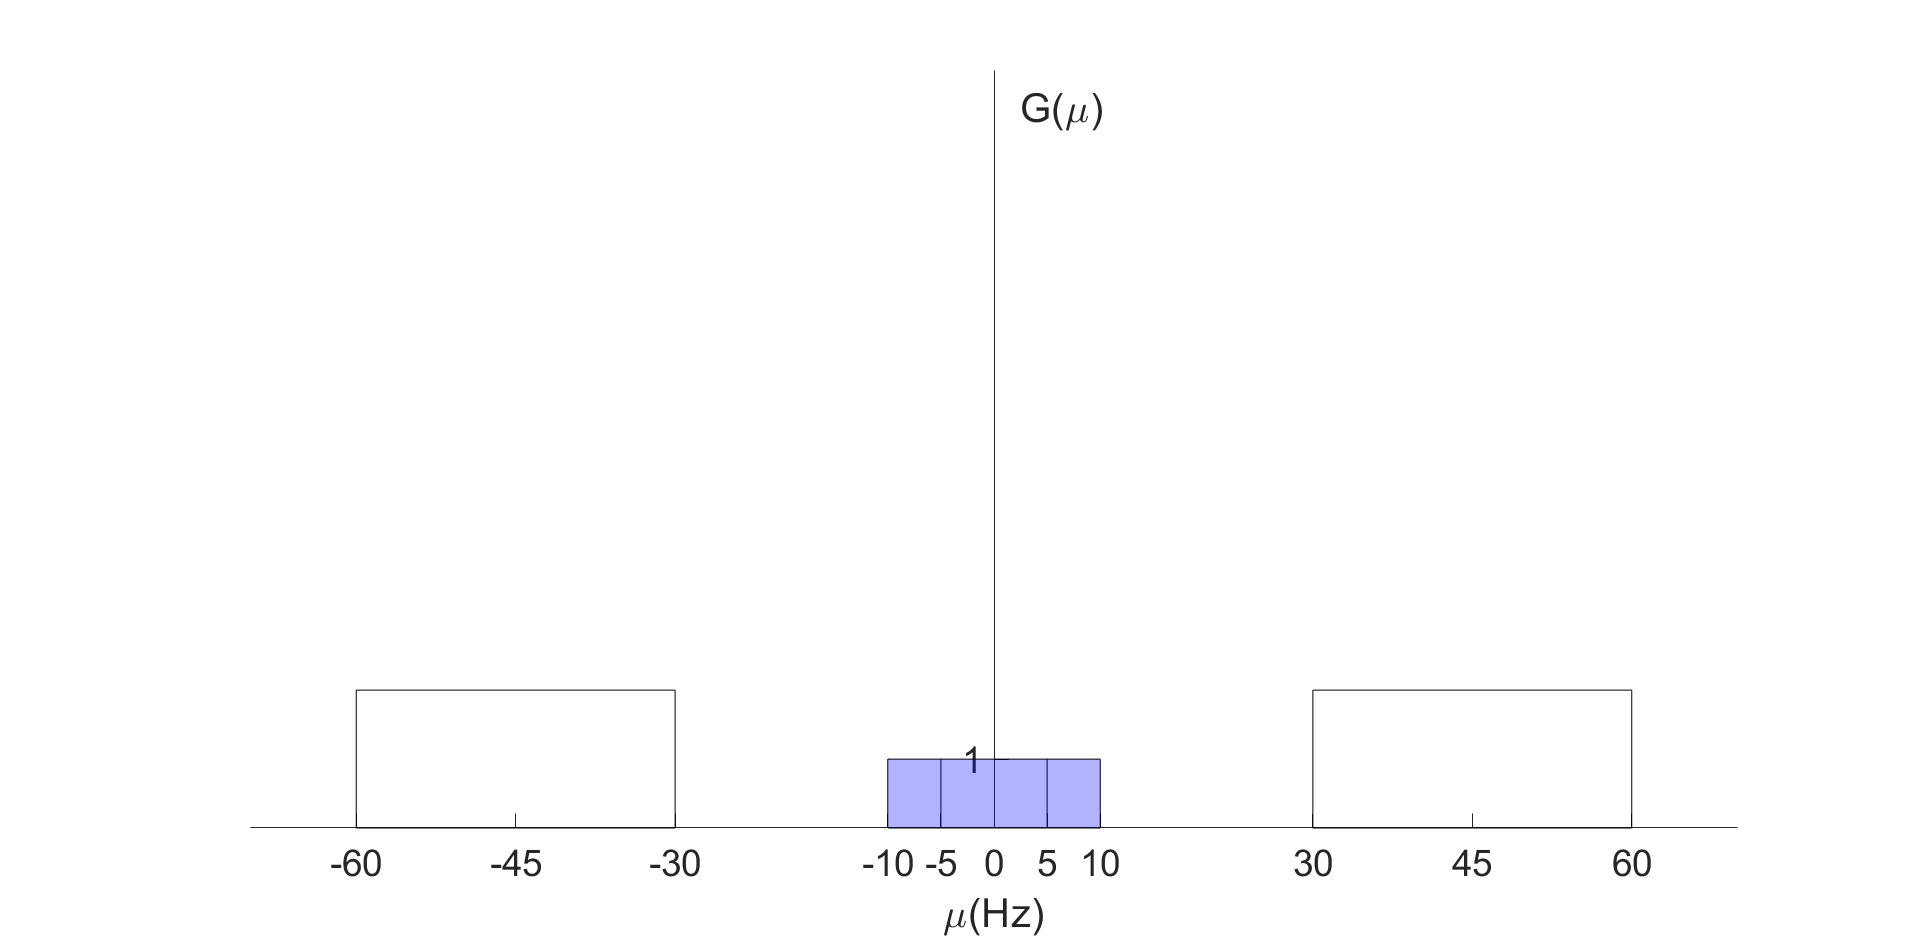
\includegraphics[width=\textwidth]{img/segnale_G.PNG}
		\caption*{Segnale $G\left(\mu\right)$.}
	\end{figure}
	
	\begin{figure}[!htp]
		\centering
		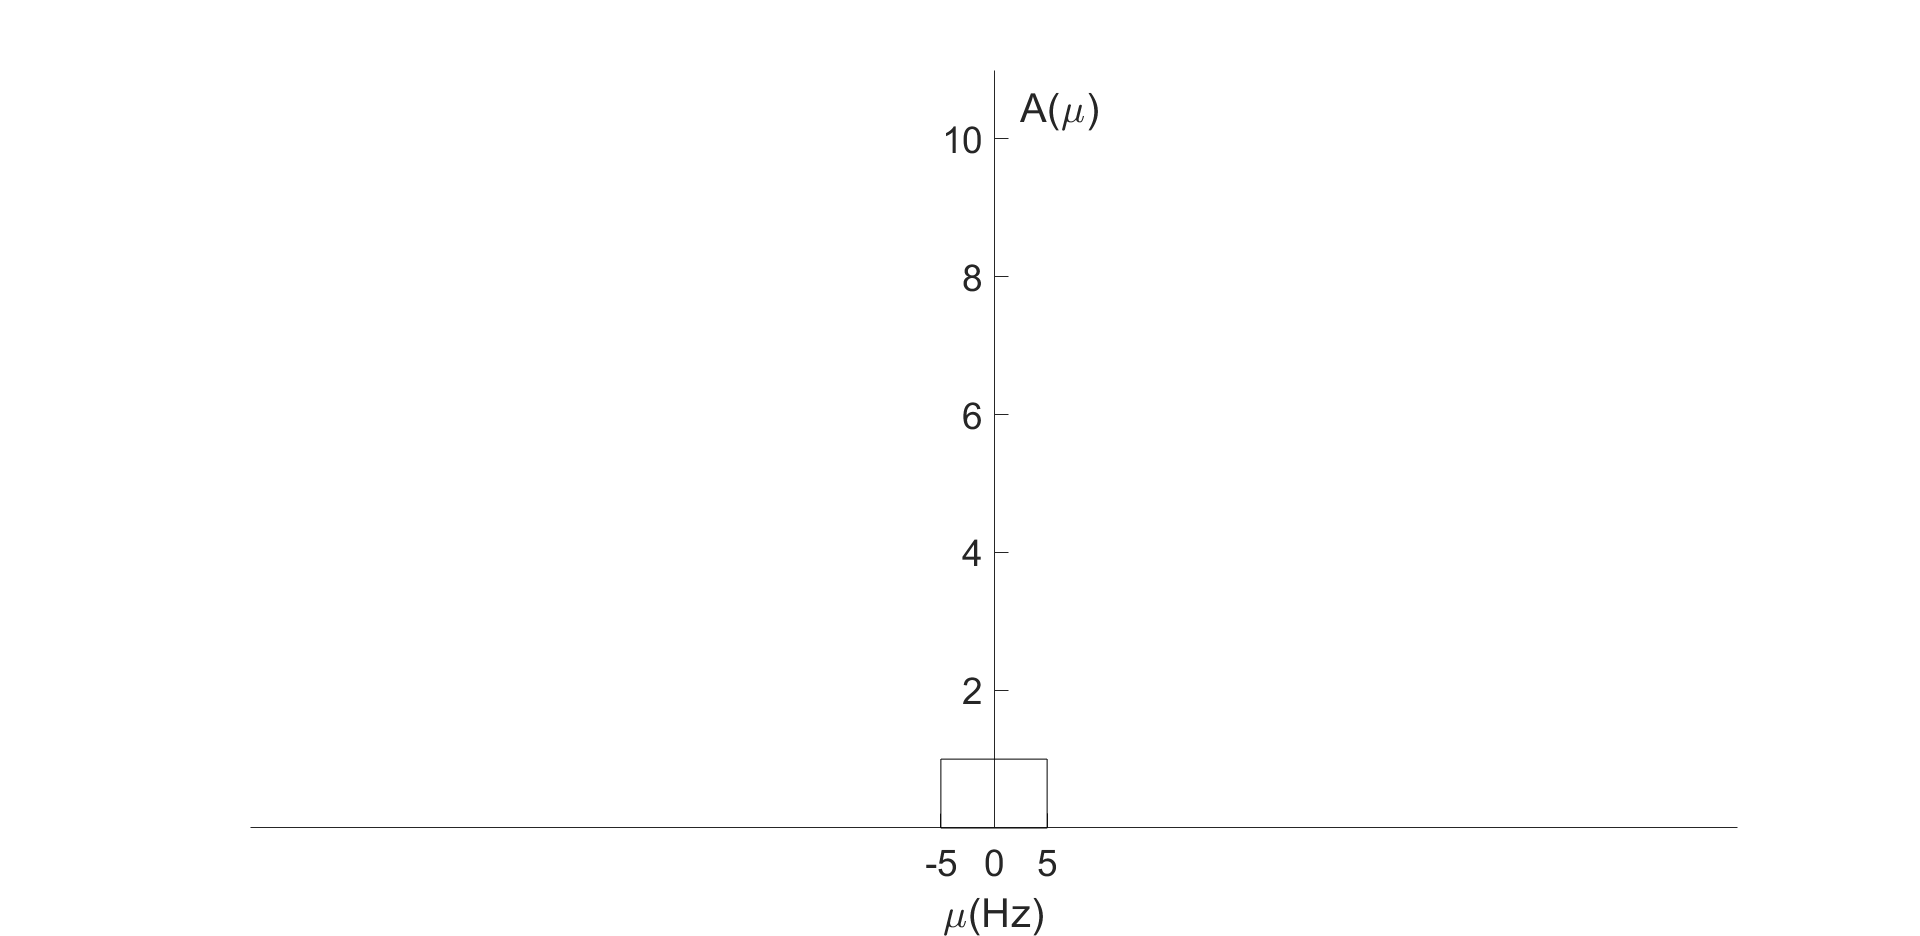
\includegraphics[width=\textwidth]{img/segnale_A.PNG}
		\caption*{Segnale $A\left(\mu\right)$ risultante.}
	\end{figure}

	\begin{figure}[!htp]
		\centering
		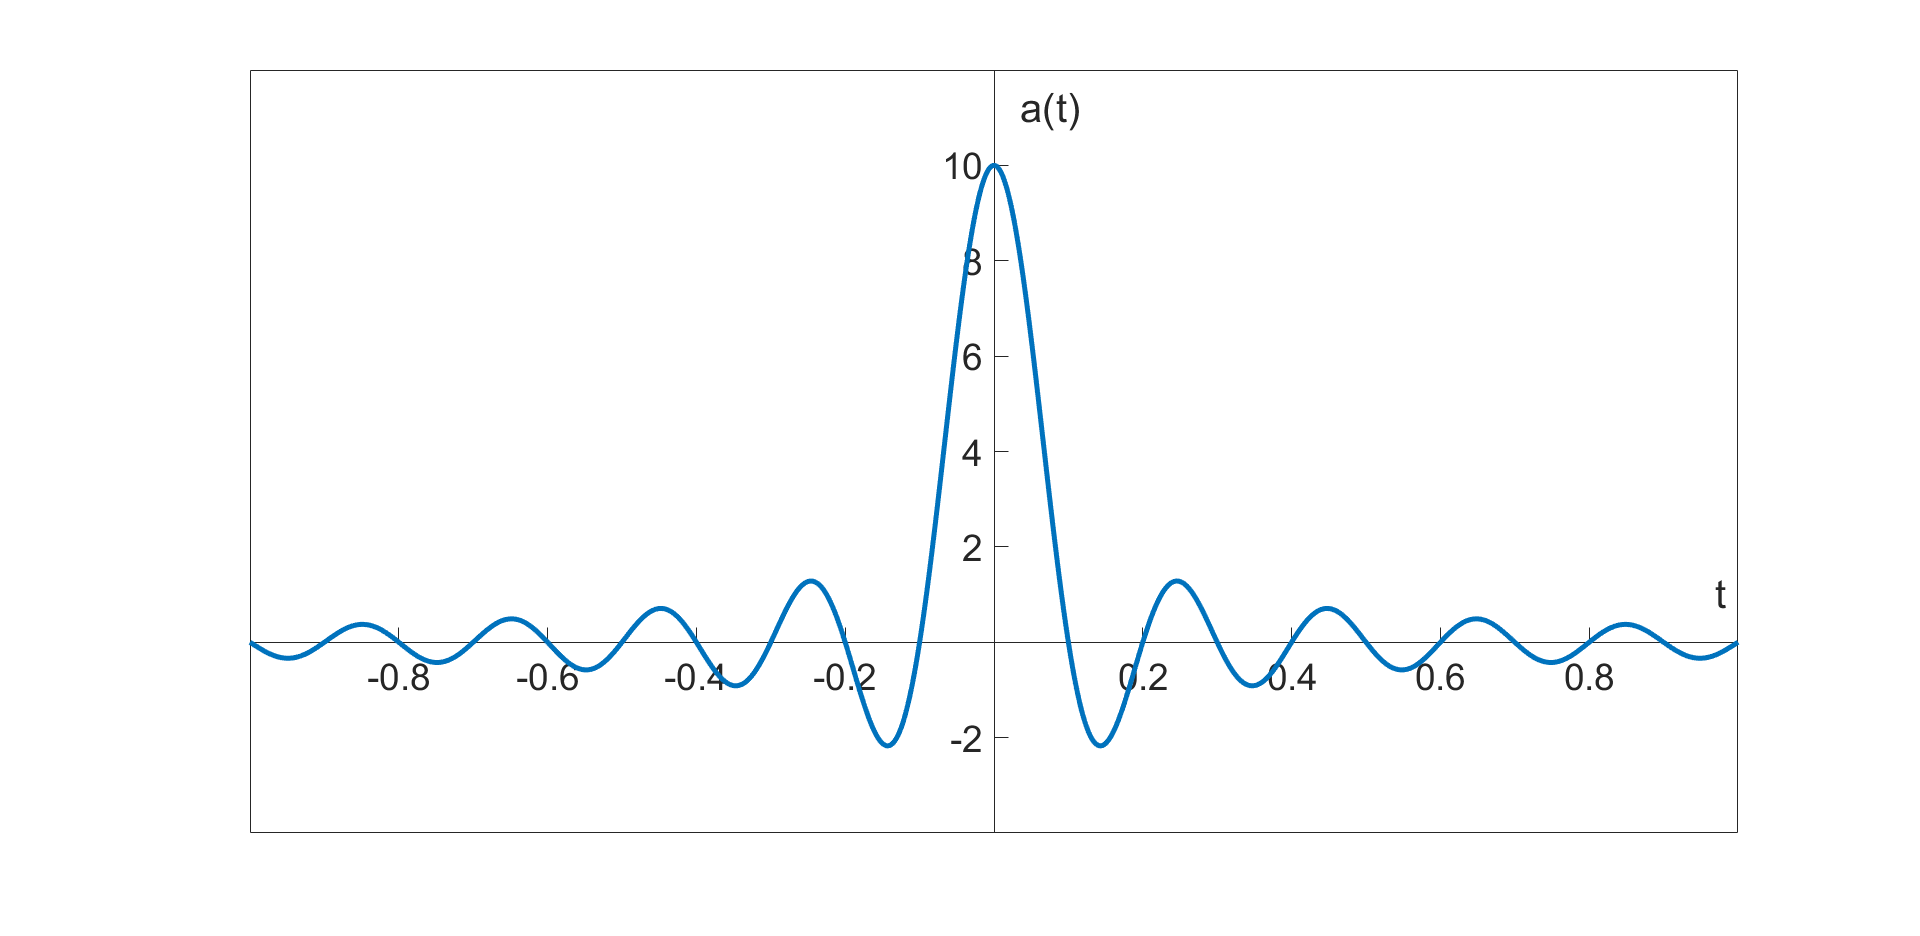
\includegraphics[width=\textwidth]{img/segnale_a-tempo.PNG}
		\caption*{Segnale nel dominio del tempo $a\left(t\right)$.}
	\end{figure}\newpage
	
	\noindent
	Adesso si esegue il \textbf{campionatore} a $10$ Hz. Attenzione: matematicamente parlando, campionare un segnale nel tempo significa moltiplicarlo per un treno di impulsi:
	\begin{equation*}
		\begin{array}{lllcl}
			\text{Dominio del tempo } & \longrightarrow & b\left(t\right) & = & a\left(t\right) \cdot \displaystyle\sum_{n = -\infty}^{\infty} \delta\left(t - \dfrac{n}{10}\right) \\
			&&&& \\
			\text{Dominio delle frequenze } & \longrightarrow & B\left(\mu\right) & = & A\left(\mu\right) * 10 \displaystyle\sum_{n = -\infty}^{\infty} \delta\left(\mu - 10n\right) \\
			&&& | & \\
			&&&=& \displaystyle\int_{-\infty}^{\infty} A\left(\tau\right) \cdot 10\displaystyle\sum_{n=-\infty}^{\infty} \delta\left(\mu - 10n - \tau\right) \mathrm{d}\tau \\
			&&&& \\
			&&& \downarrow & \text{Proprietà di setacciamento} \\
			&&&& \\
			&&&=& 10\displaystyle\sum_{n=-\infty}^{\infty} A\left(\mu - 10n\right) \\
			&&& | & \\
			&&&=& 10\displaystyle\sum_{n=-\infty}^{\infty} G\left(\mu - 10n\right) \cdot \Pi\left(\dfrac{\mu - 10n}{20}\right) \\
		\end{array}
	\end{equation*}
	\begin{figure}[!htp]
		\centering
		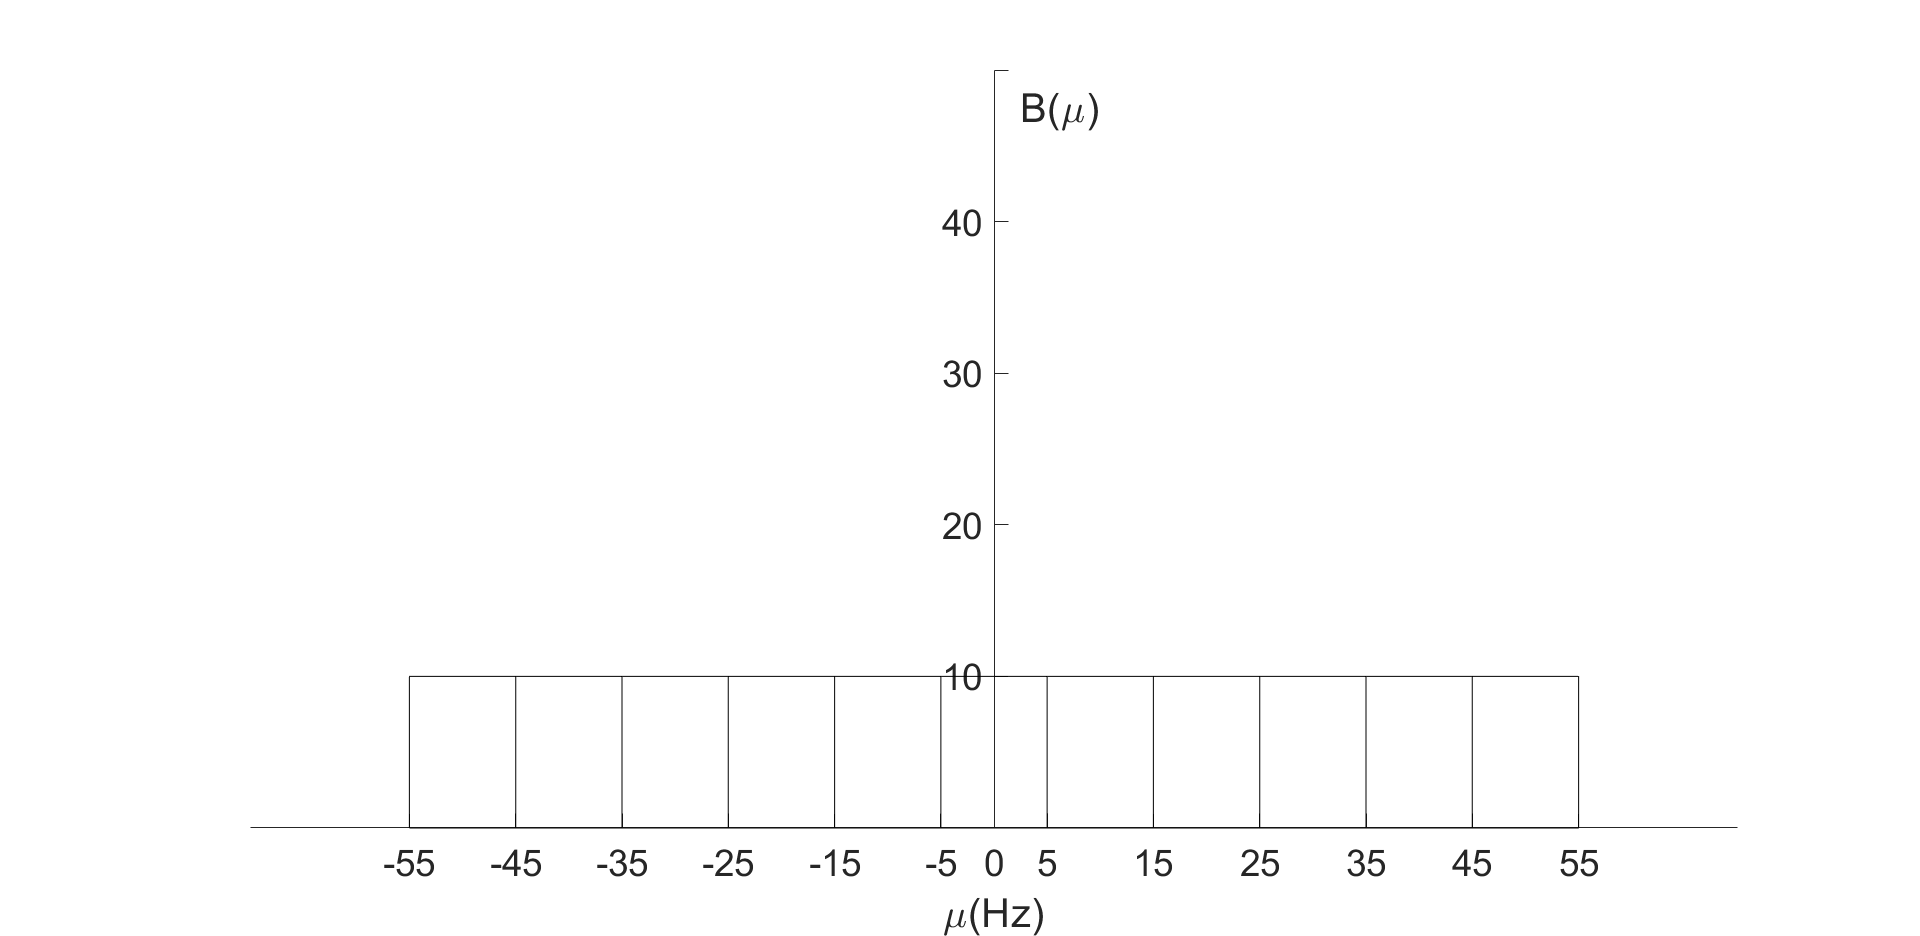
\includegraphics[width=\textwidth]{img/segnale_A-campionatore.PNG}
		\caption*{Il segnale $A\left(\mu\right)$ viene ripetuto ogni $10$ Hz.\newline
			\textbf{\underline{Attenzione}}: non c'è aliasing poiché non c'è sovrapposizione ma appaiamento.}
	\end{figure}\newpage

	\begin{figure}[!htp]
		\centering
		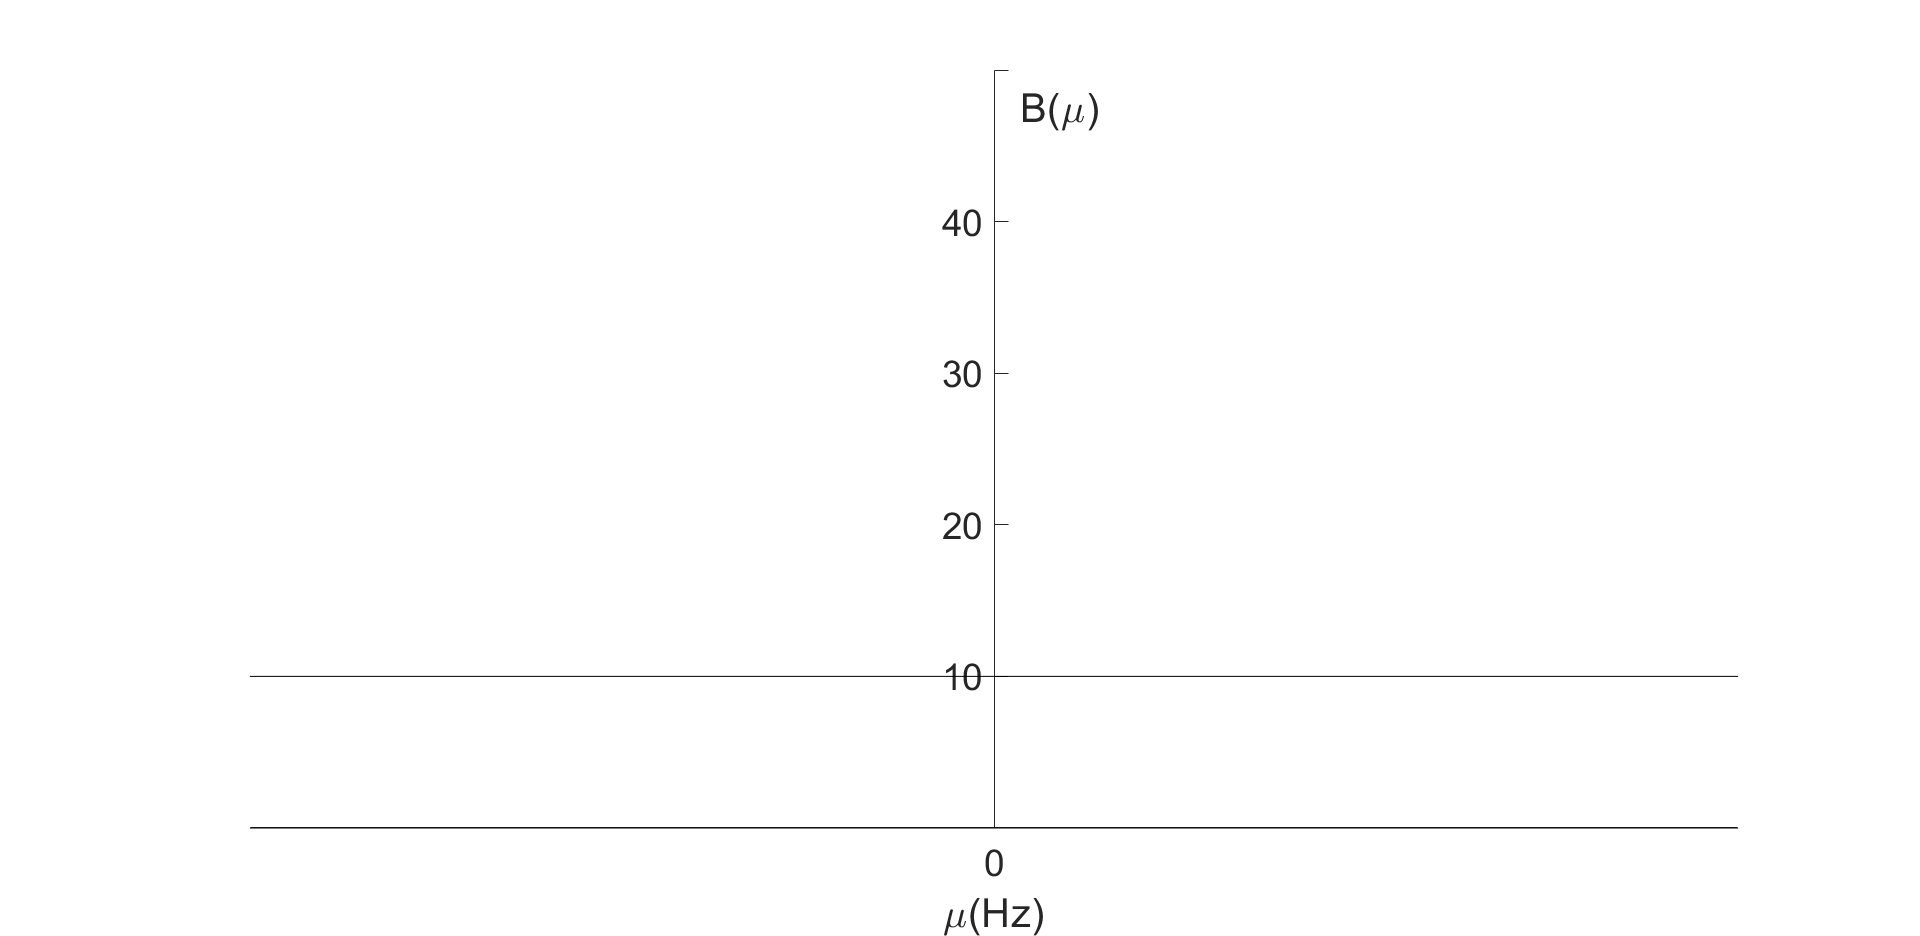
\includegraphics[width=\textwidth]{img/segnale_B.PNG}
		\caption*{Il segnale $B\left(\mu\right)$ risultante è costante a $10$.}
	\end{figure}
	
	\begin{figure}[!htp]
		\centering
		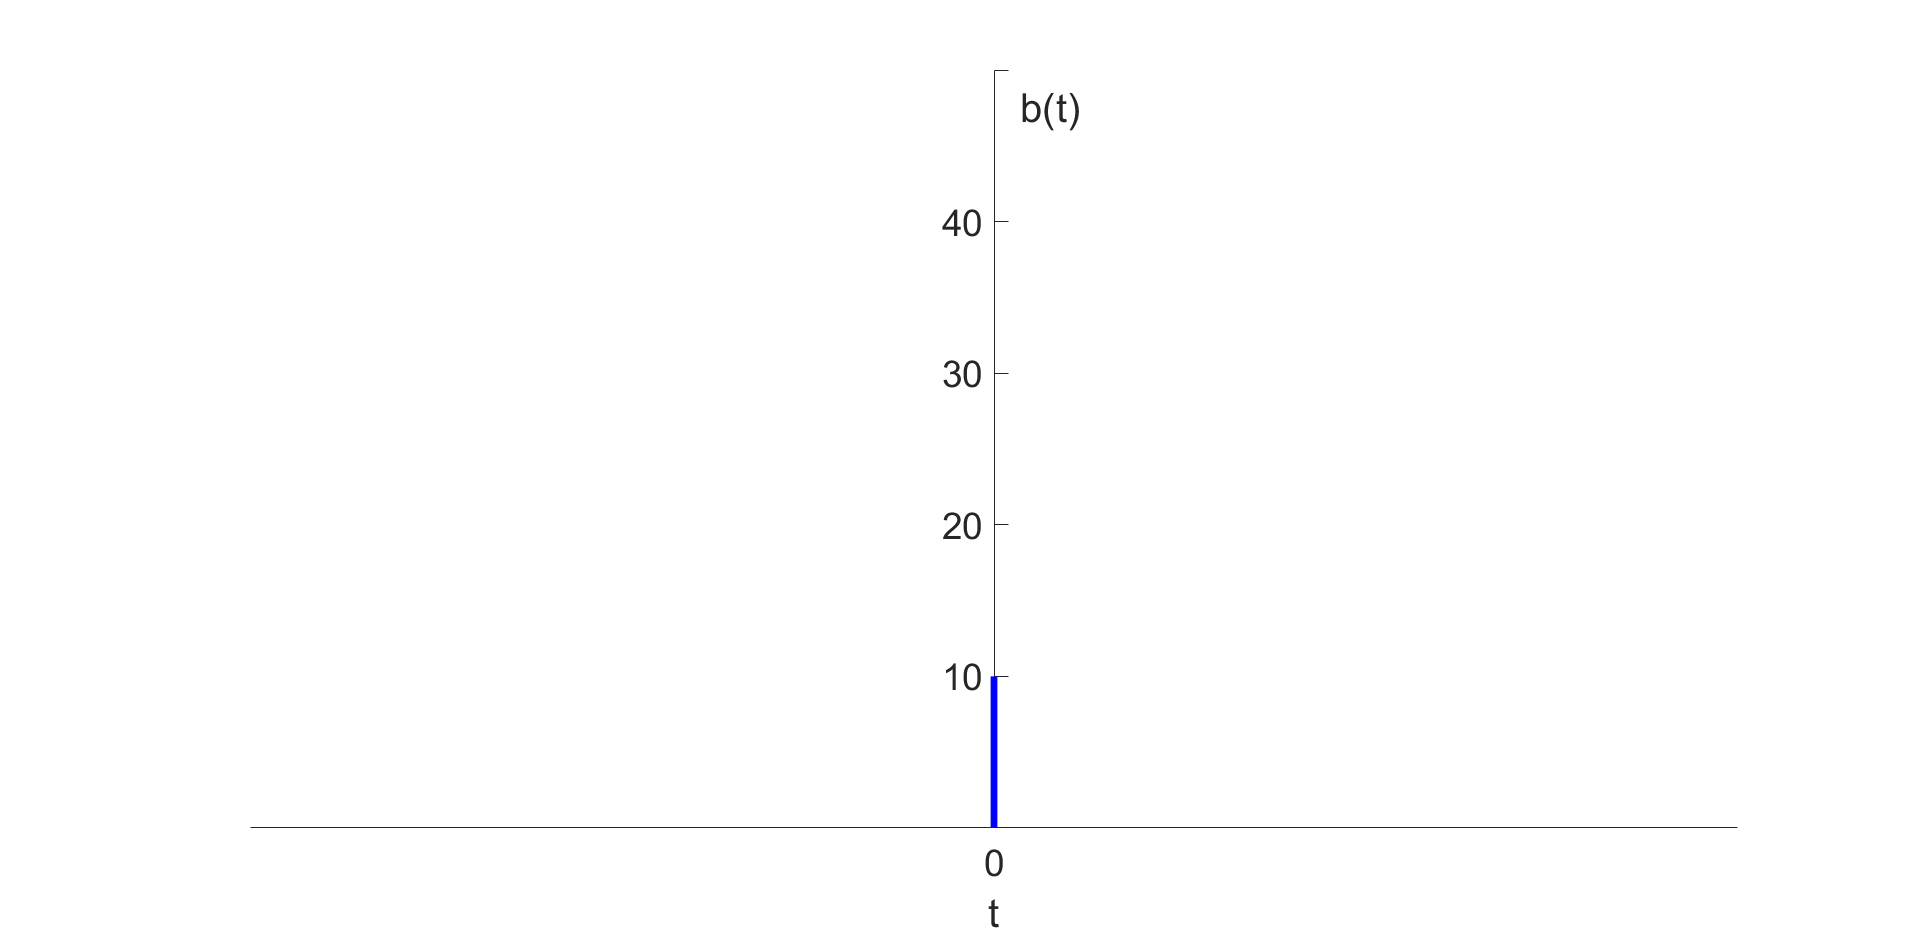
\includegraphics[width=\textwidth]{img/segnale_b-tempo.PNG}
		\caption*{Segnale nel dominio del tempo $b\left(t\right)$.}
	\end{figure}\newpage

	\noindent
	Infine, si applica l'ultimo filtro \textbf{passa basso ideale} con frequenza di taglio $25$~Hz:
	\begin{equation*}
		\begin{array}{lll}
			\text{Dominio del tempo } & \longrightarrow & c\left(t\right) = b\left(t\right) * 50\mathrm{sinc}\left(50t\right) \\
			&& \\
			\text{Dominio delle frequenze } & \longrightarrow & C\left(\mu\right) = B\left(\mu\right) \cdot \Pi\left(\dfrac{\mu}{50}\right)
		\end{array}
	\end{equation*}
	
	\begin{figure}[!htp]
		\centering
		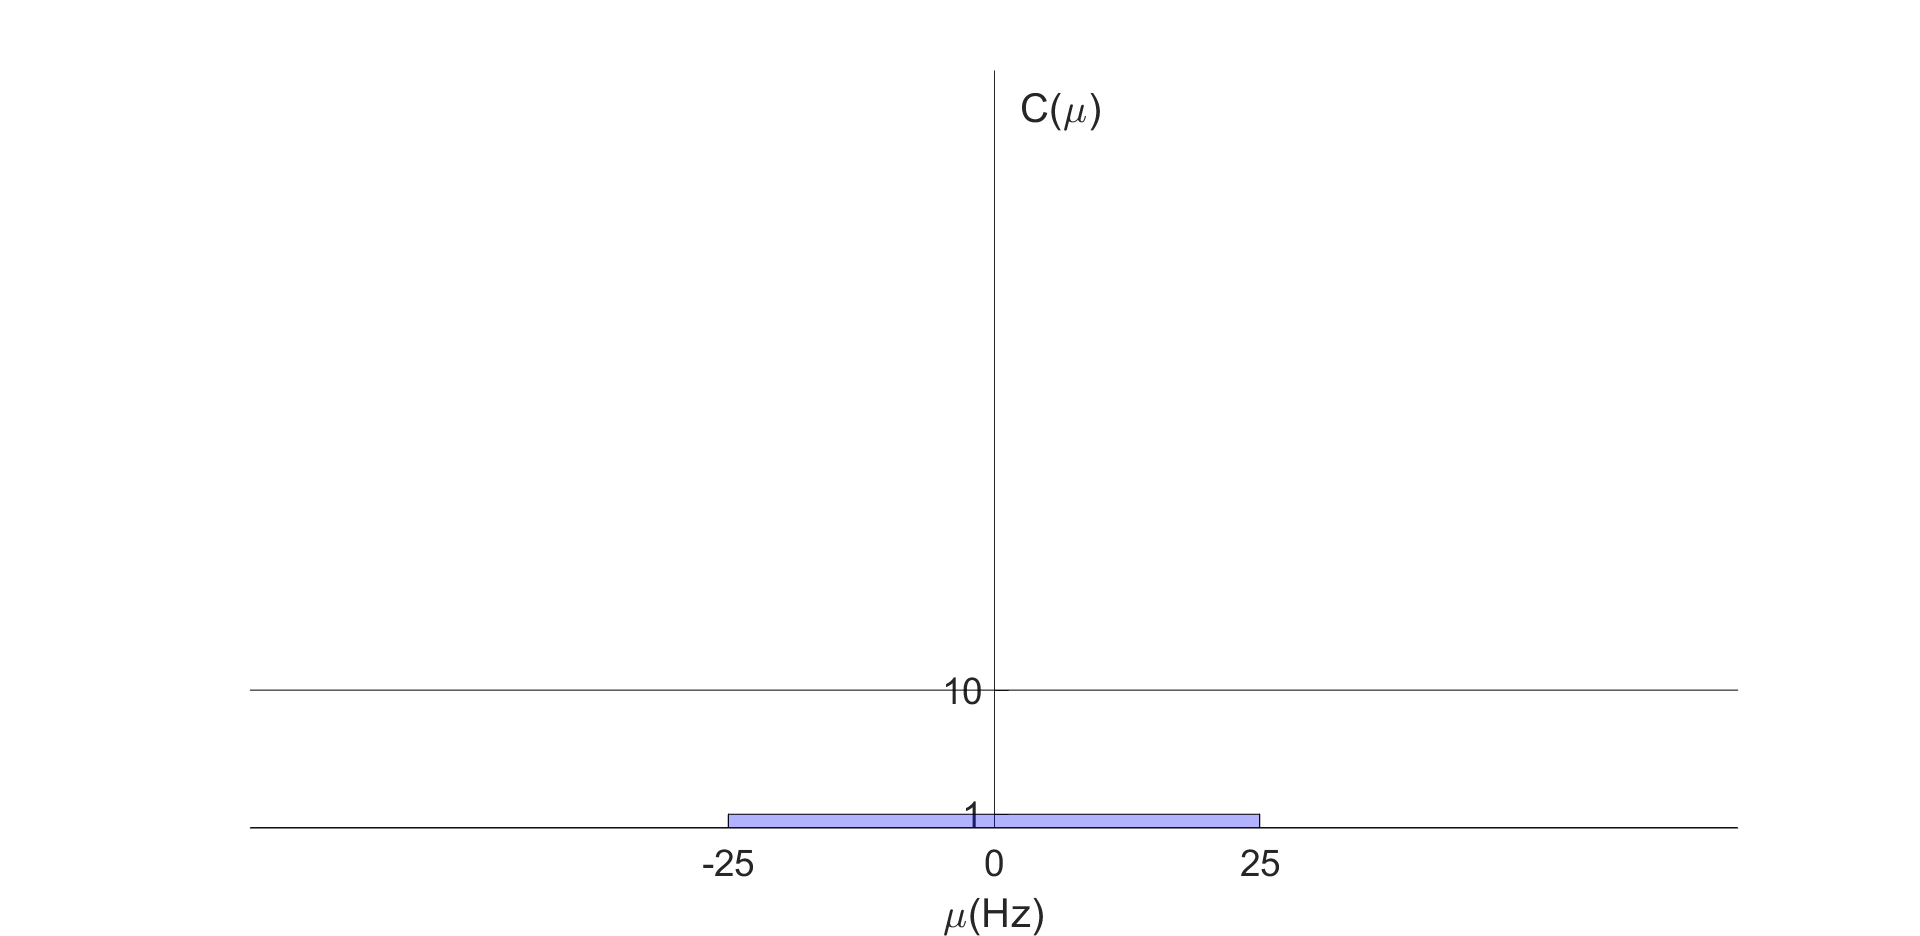
\includegraphics[width=\textwidth]{img/segnale_B-con-filtro.PNG}
		\caption*{Segnale $B\left(\mu\right)$ con il filtro passa basso ideale.}
	\end{figure}
	
	\begin{figure}[!htp]
		\centering
		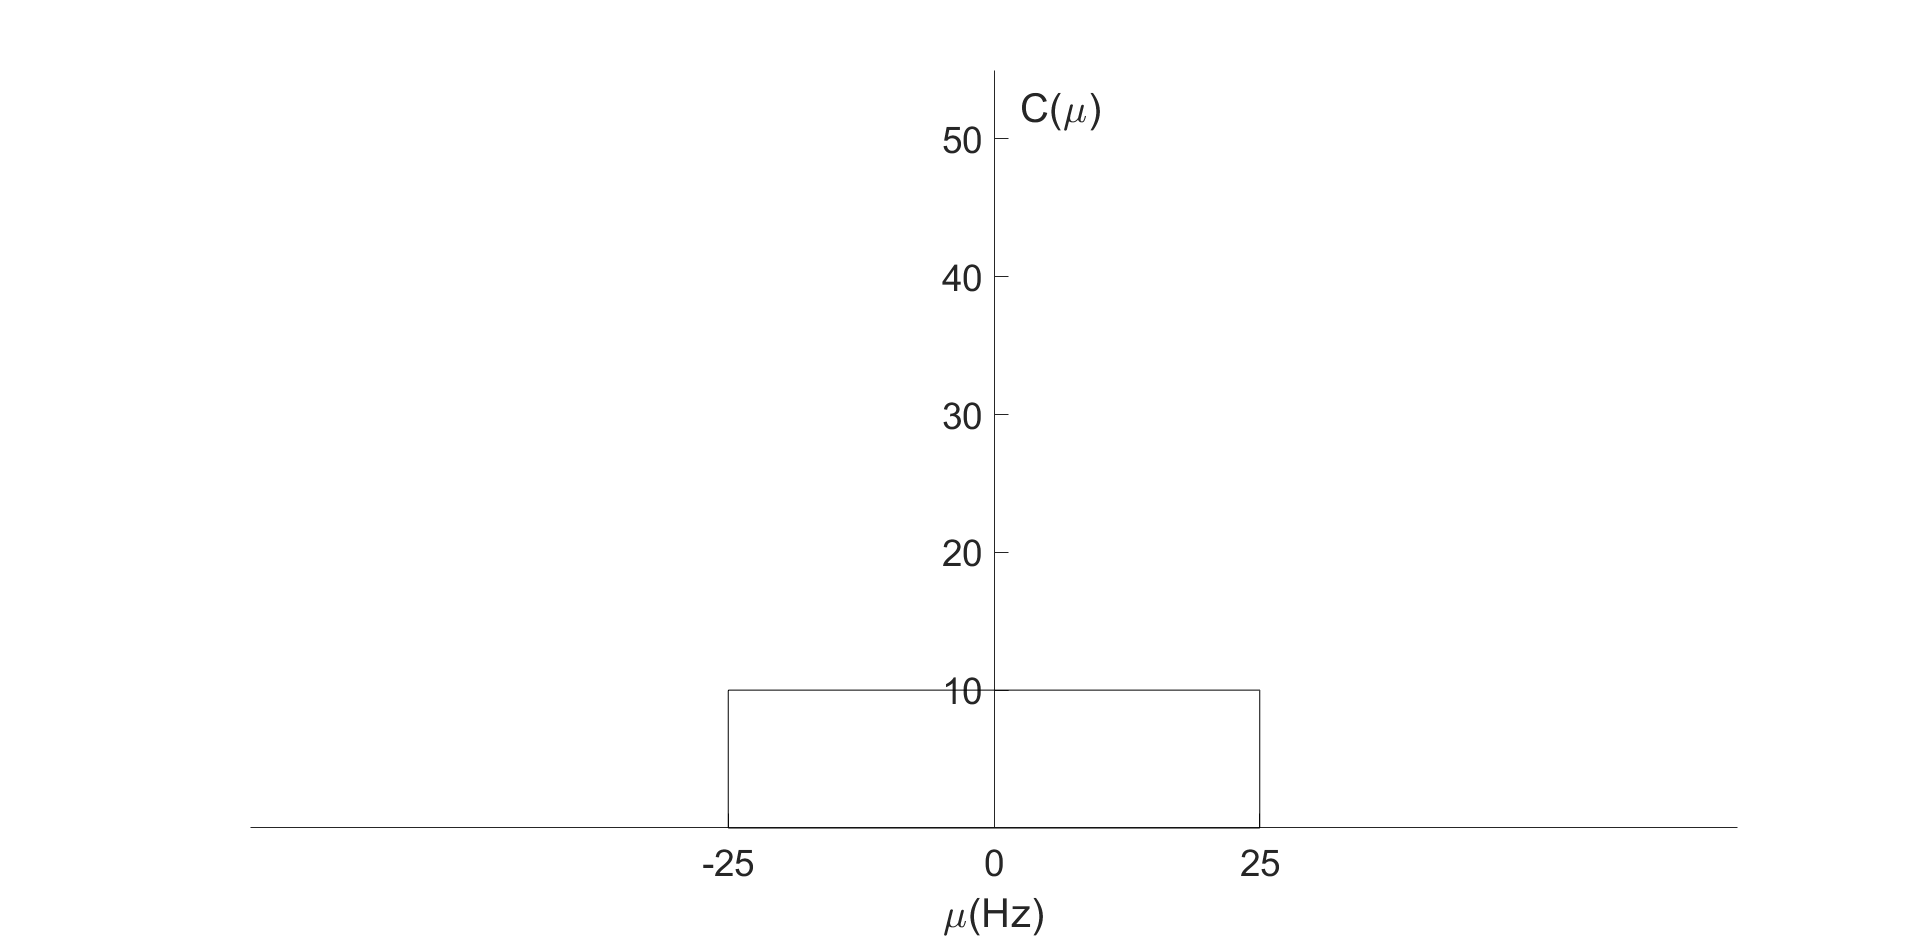
\includegraphics[width=\textwidth]{img/segnale_C.PNG}
		\caption*{Segnale $C\left(\mu\right)$ risultante.}
	\end{figure}\newpage
	
	\begin{figure}[!htp]
		\centering
		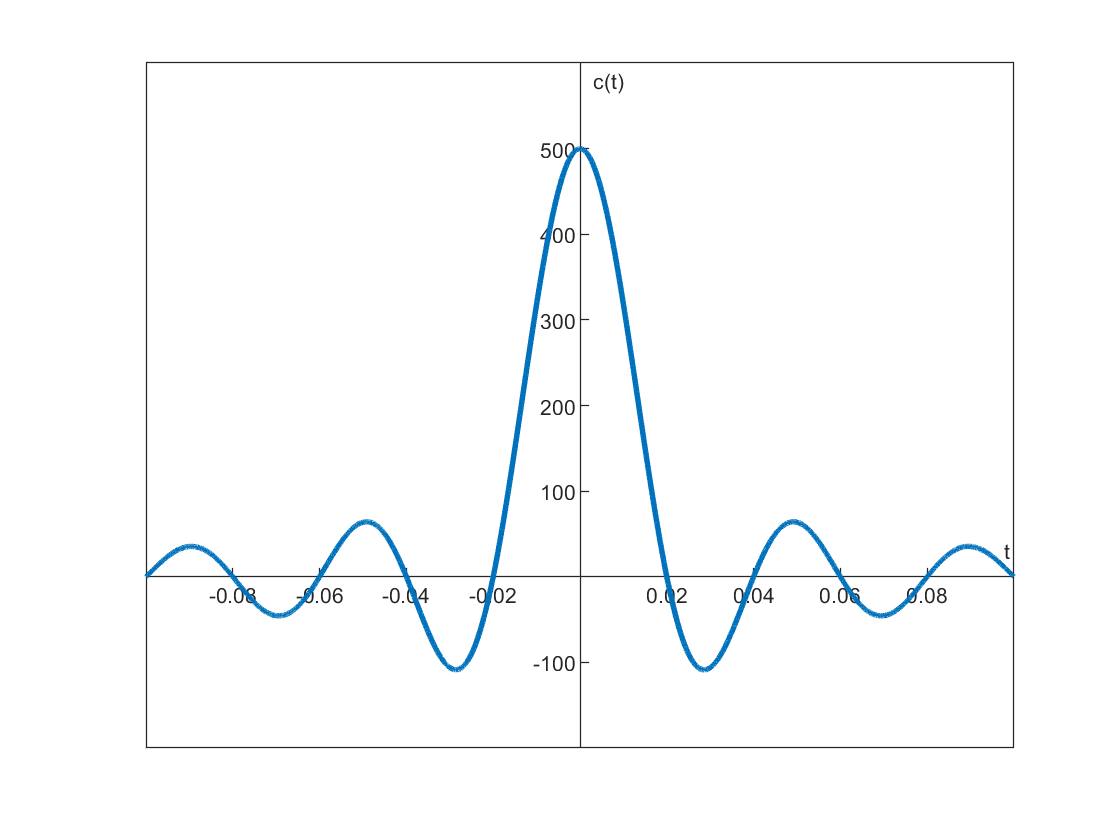
\includegraphics[width=\textwidth]{img/segnale_c-tempo.PNG}
		\caption*{Segnale nel dominio del tempo $c\left(t\right)$.}
	\end{figure}\newpage
	
	\section{Soluzione Esercizio (7 punti)}
	\subsection*{Fonte: Simulazione 15/01/2021}
	
	Si traducono i segnali rappresentati graficamente in funzioni nel dominio continuo del tempo:
	\begin{equation*}
		\begin{array}{lll}
			x\left(t\right) & = & 2 \Pi \left(\dfrac{t-1}{2}\right) \\
			&& \\
			h\left(t\right) & = & \delta\left(t-1\right) + \delta\left(t-2\right)
		\end{array}
	\end{equation*}
	Si calcola il segnale $y\left(t\right)$ eseguendo la convoluzione tra i due segnali:
	\begin{equation*}
		\begin{array}{lcl}
			y\left(t\right)	& = & x\left(t\right) * h\left(t\right) \\
							& | & \\
							& = & \displaystyle\int_{-\infty}^{\infty} x\left(\tau\right) \cdot \left[\delta\left(t - 1 - \tau\right) + \delta\left(t - 2 - \tau\right)\right] \mathrm{d}\tau \\
							& | & \\
							& = & \displaystyle\int_{-\infty}^{\infty} x\left(\tau\right) \delta\left(t - 1 - \tau\right) + x\left(\tau\right)\delta\left(t - 2 - \tau\right) \mathrm{d}\tau \\
							&  & \\
							& \downarrow & \text{Proprietà di setacciamento} \\
							&  & \\
							& = & x\left(t-2\right) + x\left(t-1\right) \\
							& | & \\
							& = & 2\Pi\left(\dfrac{t - 1 -1}{2}\right) + 2\Pi\left(\dfrac{t - 2 - 1}{2}\right) \\
							& | & \\
							& = & 2\Pi\left(\dfrac{t-2}{2}\right) + 2\Pi\left(\dfrac{t-3}{2}\right)
		\end{array}
	\end{equation*}\newpage
	La convoluzione grafica tra i due segnali $x\left(t\right)$ e $h\left(t\right)$ è la seguente:
	\begin{figure}[!htp]
		\centering
		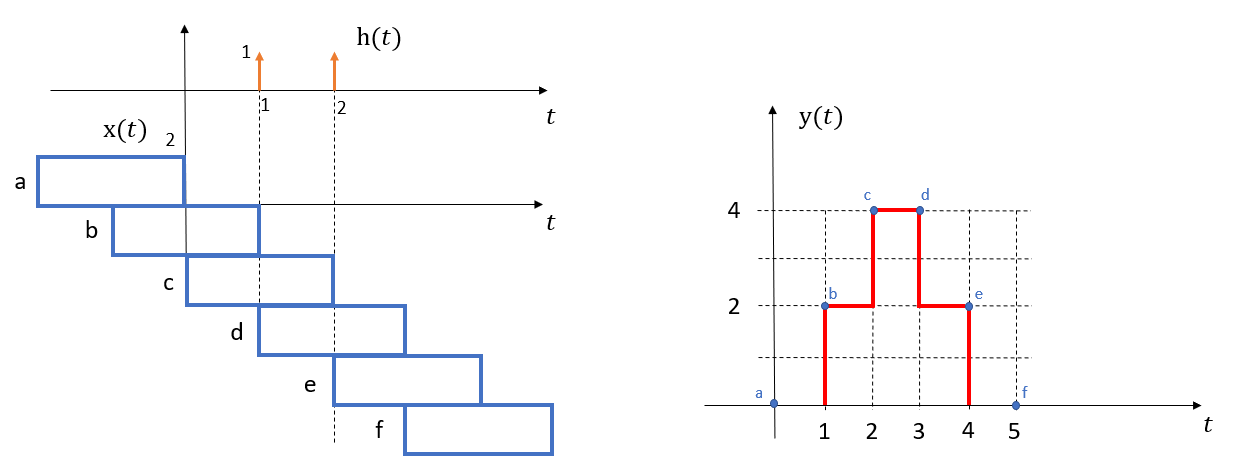
\includegraphics[width=\textwidth]{img/convoluzione.PNG}
	\end{figure}
	\begin{enumerate}[label=\alph*.]
		\item Non c'è intersezione tra i segnali, $y$ in $0$ non esiste;
		\item C'è intersezione, il prodotto tra i segnali è un impulso di ampiezza $2$, $y\left(1\right) = 2$;
		\item C'è intersezione, il prodotto tra i segnali produce due impulsi di ampiezza $2$ ciascuno, l'integrale del prodotto vale $4$, $y\left(2\right) = 4$;
		\item C'è intersezione, il prodotto tra i segnali produce due impulsi di ampiezza $2$ ciascuno, l'integrale del prodotto vale $4$, $y\left(3\right) = 4$;
		\item C'è intersezione, il prodotto tra i segnali è un impulso di ampiezza $2$, $y\left(4\right) = 2$.
		\item Non ci può più essere intersezione tra i segnali poiché $y$ in $0$ non esiste.
	\end{enumerate}\newpage

	\section{Soluzione Esercizio (7 punti)}
	\subsection*{Fonte: Slide del corso}

	Le risposte alle domande sono elencate qua di seguito. La prima risposta cerca di coprire entrambe le risposte sul \emph{ringing}:
	\begin{itemize}
		\item Il \emph{\textbf{ringing}}, o effetto di Gibbs, è un effetto visivo causato dall'applicazione di un filtro passa basso ideale (in frequenza), ovvero dell'esecuzione di una convoluzione con l'operatore $\mathrm{sinc}$ (nello spazio). Quindi, la risposta all'impulso del filtro passa basso ideale è ancora un $\mathrm{sinc}$ e l'immagine visivamente risulta increspata vicino ai bordi taglienti (effetto ringing).\newline
		\begin{figure}[!htp]
			\centering
			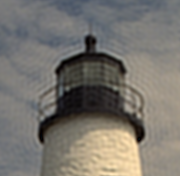
\includegraphics[width=.4\textwidth]{img/ringing.PNG}
			\caption*{Effetto \emph{ringing} su un'immagine.}
		\end{figure}
	
		\noindent
		Per quanto il filtro passa basso \underline{ideale} sia una delle cause maggiori, anche il filtro passa basso di Butterworth ha la caratteristica di creare \emph{ringing}. Ma questo avviene solamente per ordini elevati, dunque è evitabile talvolta.\newline
		Una \textbf{soluzione} adottabile, ma non sempre disponibile, è quella di applicare un filtro di passa basso diverso da quello ideale. Per esempio, un'ottima scelta sarebbe un filtro passa basso Gaussiano che non crea nessun fenomeno di \emph{ringing}. Certo è che non sarà mai ottimo come un filtro passa basso ideale, questo perché esso provoca un altro effetto indesiderato chiamato \emph{blur} (offuscamento).\newline
		Il filtro passa basso Gaussiano non presenta \emph{ringing} poiché non è mai negativa e non presenta oscillazioni. Si lascia qua sotto un confronto tra il grafico nel dominio del tempo di un filtro passa basso \underline{ideale} e \underline{Gaussiano} per comprendere meglio questo concetto.\newpage
		\begin{figure}[!htp]
			\centering
			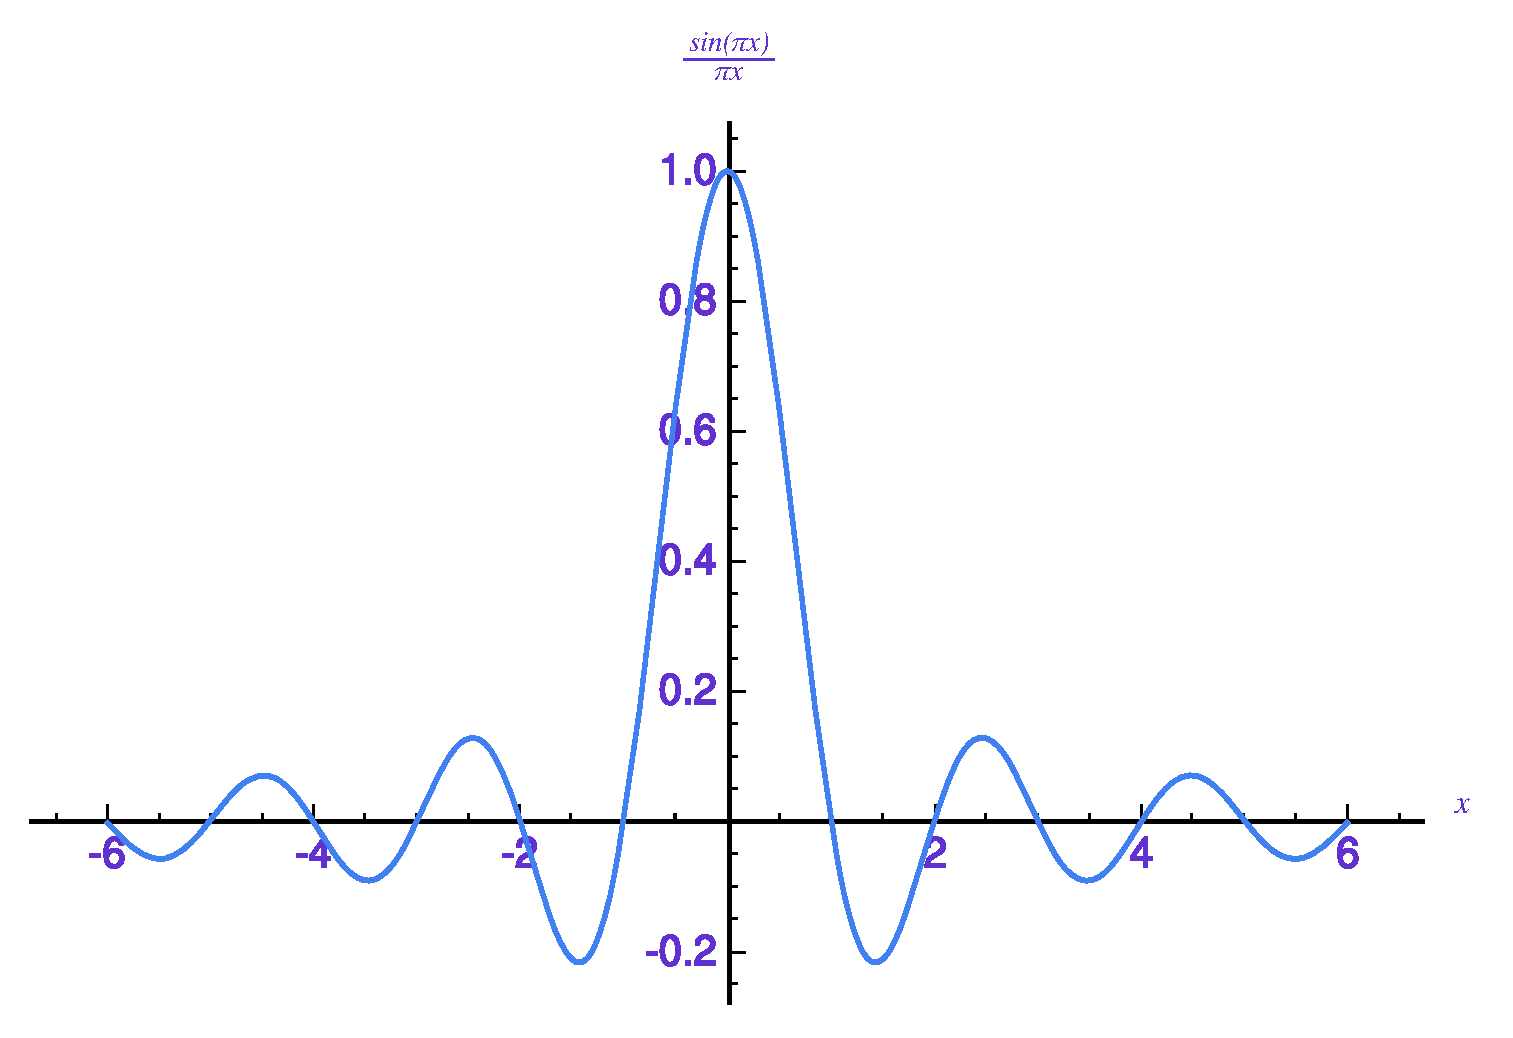
\includegraphics[width=.8\textwidth]{img/filtro_passa_basso_ideale.pdf}
			\caption*{Rappresentazione grafica di un filtro passa basso ideale nel tempo. Si noti l'oscillazione e la presenza di valori negativi.}
		\end{figure}
		
		\begin{figure}[!htp]
			\centering
			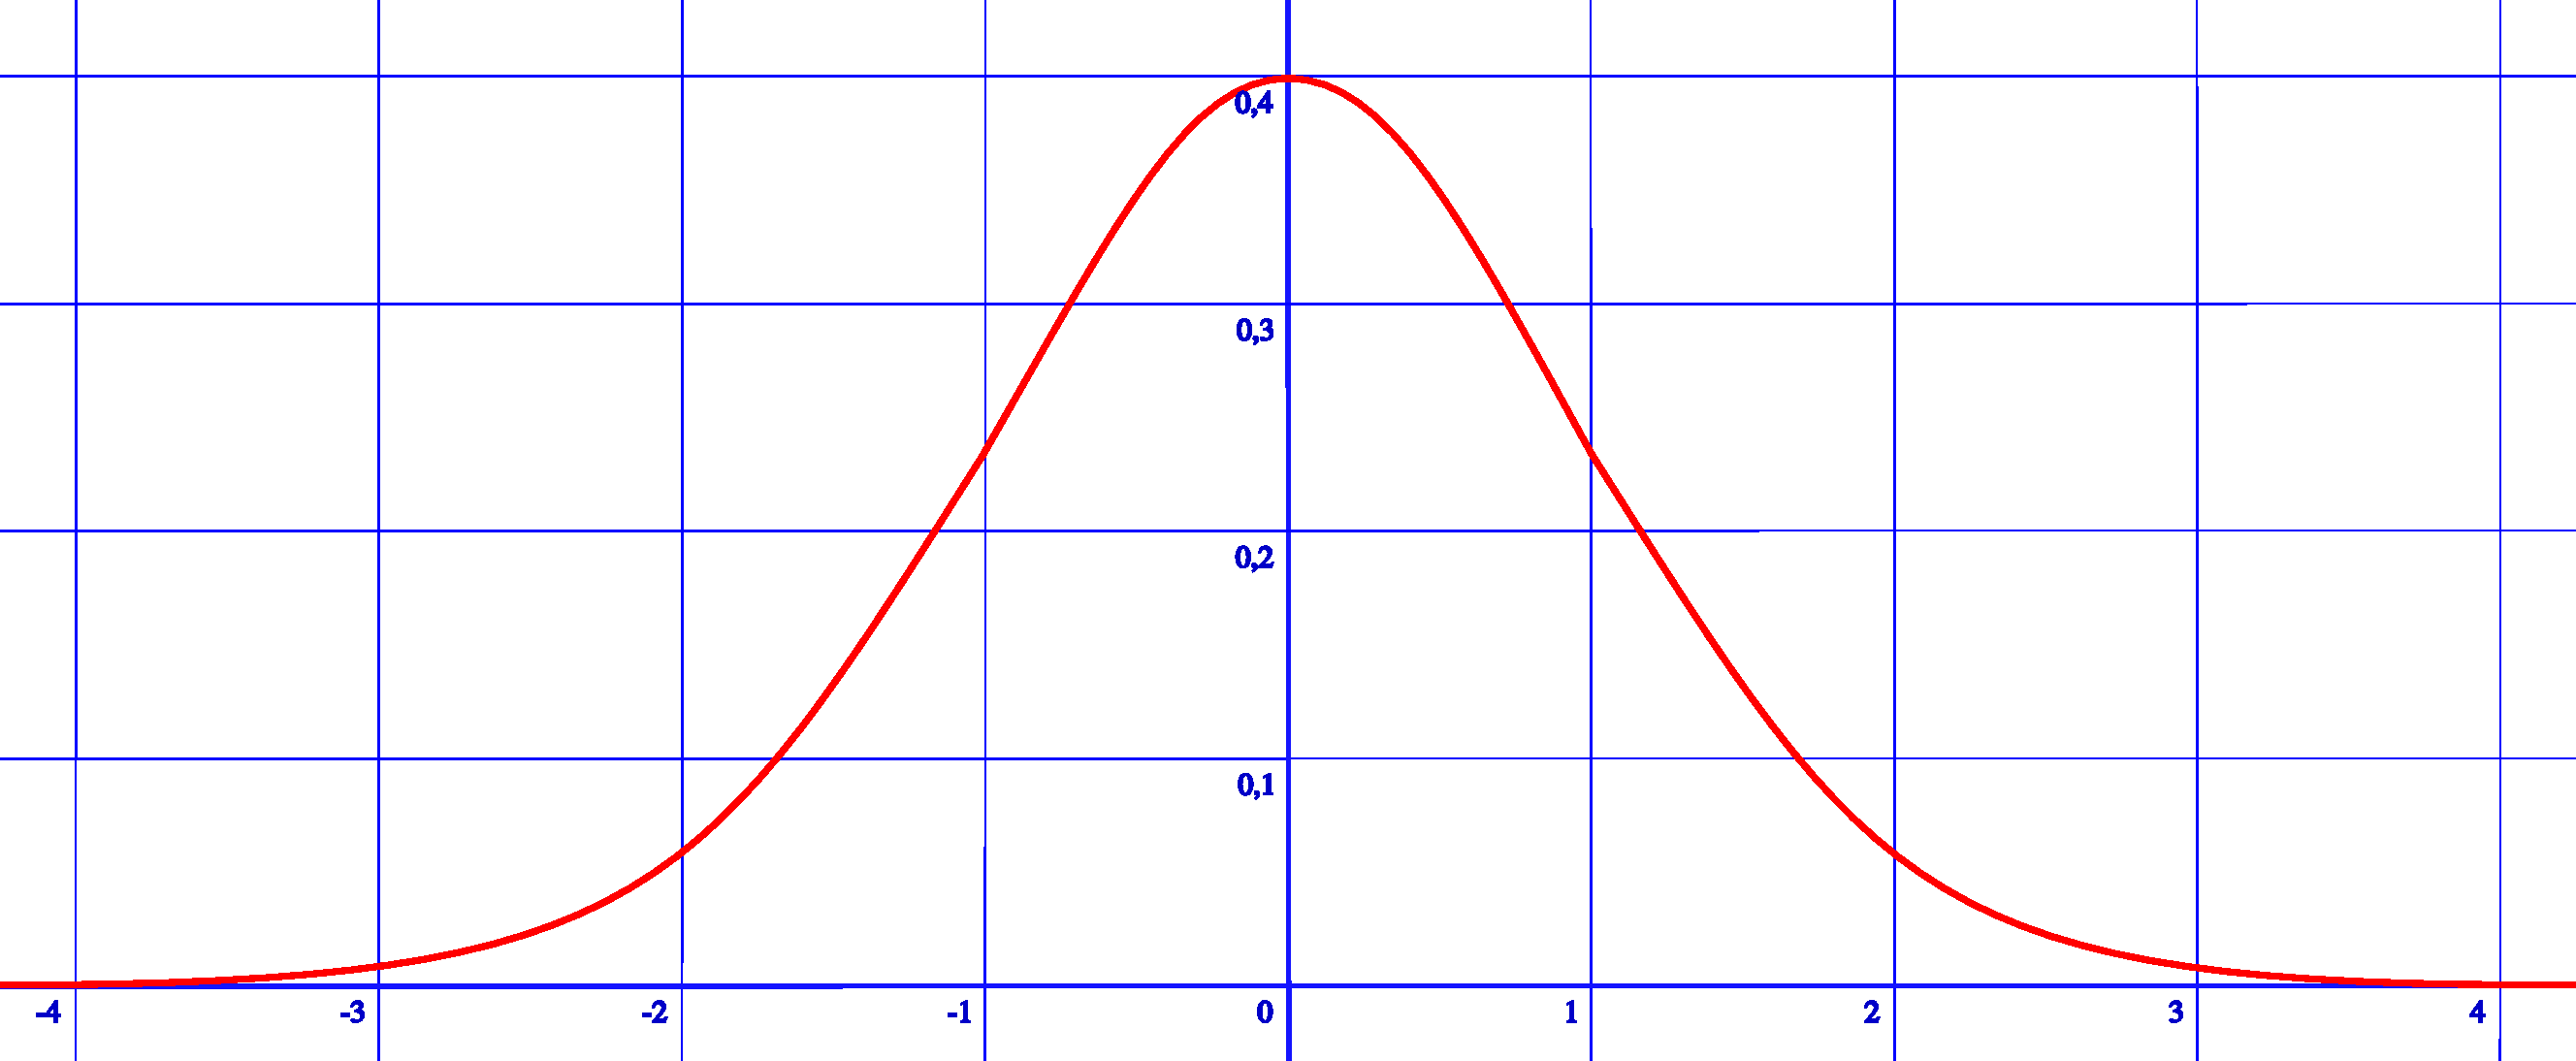
\includegraphics[width=.8\textwidth]{img/gaussiana.pdf}
			\caption*{Rappresentazione grafica di un filtro passa basso Gaussiano nel tempo. Si noti l'oscillazione assente e valori solo positivi o nulli.}
		\end{figure}\newpage
	
		\item Un \textbf{filtro passa basso ideale} viene utilizzato per ottenere: lo sfocamento e lo \emph{smoothing}. Matematicamente parlando, esso è una funzione di trasferimento, uguale alla sua trasformata nel dominio delle frequenze, di una box.\newline
		Il termine \textbf{ideale} è dovuto alla transizione rapida in corrispondenza alla frequenza di taglio. Come si vede dall'immagine, un cambio così repentino non è analogicamente realizzabile.\newline
		In parole povere, è ideale poiché nell'elettronica non può fisicamente avvenire un cambio di energia così repentino.\newline
		\begin{figure}[!htp]
			\centering
			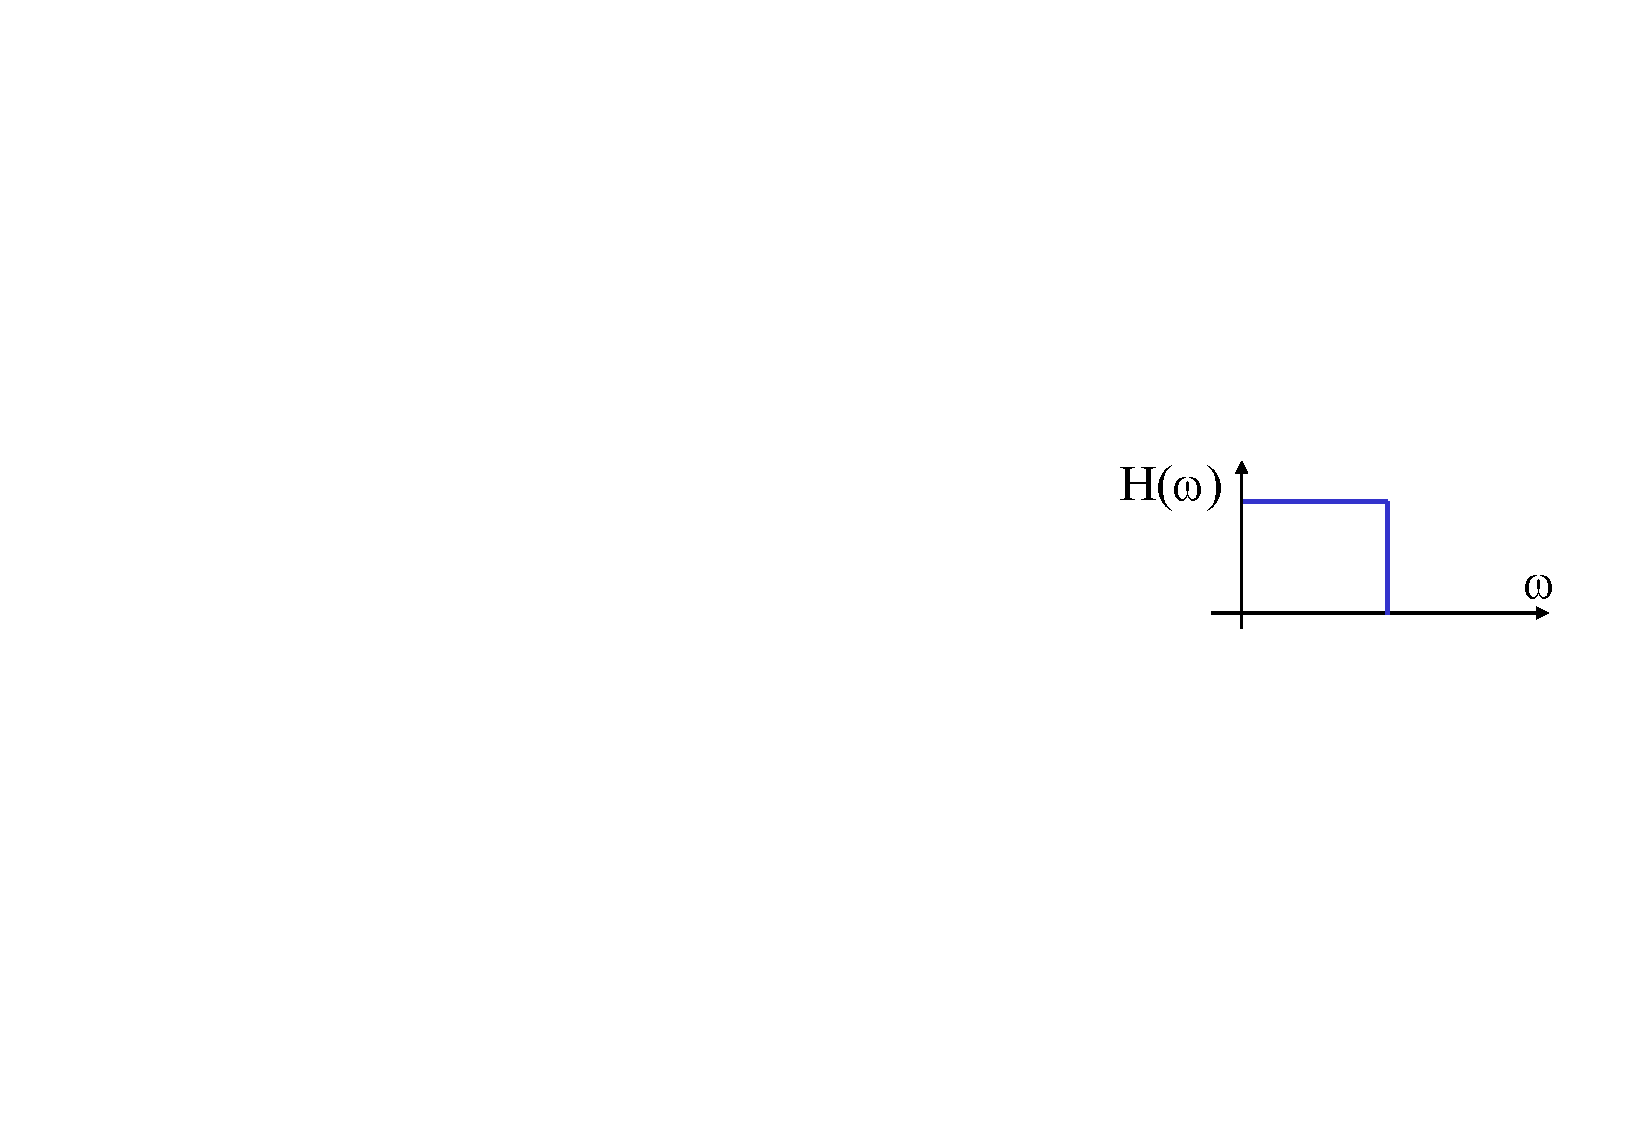
\includegraphics[width=.35\textwidth]{img/box_filtro_passa_bassa_ideale.pdf}
		\end{figure}
			
		\noindent
		Si rappresenta graficamente un filtro passa basso ideale con frequenze $15$ e $25$ Hz:
		\begin{figure}[!htp]
			\centering
			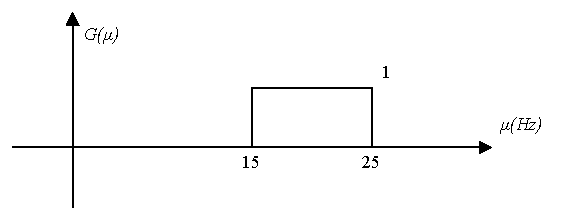
\includegraphics[width=.8\textwidth]{img/filtro_passa_basso_ideale_ex.pdf}
		\end{figure}
		
		\noindent
		E analiticamente:
		\begin{equation*}
			\begin{array}{lll}
				\text{Dominio delle frequenze } & \longrightarrow & G\left(\mu\right) = \Pi\left(\dfrac{\mu - 20}{10}\right) \\
				&& \\
				\text{Dominio del tempo } & \longrightarrow & g\left(t\right) = 10\mathrm{sinc}\left(10t\right) \cdot e^{-j 2 \pi t 20}
			\end{array}
		\end{equation*}
	\end{itemize}\newpage
	
	\section{Soluzione Esercizio (6 punti)}
	\subsection*{Fonte: Lezione 6 di laboratorio}
	
	Il codice implementa l'operazione puntuale di clamping. Essa viene utilizzata nel caso in cui ci siano dei pixel di rumore molto chiari o molto scuri che mascherano l'immagine. Per esempio, un'immagine con dei puntini bianchi può essere migliorata utilizzando questa operazione puntuale.\newline
	
	\noindent
	Il codice MATLAB presenta degli errori con gli indici. Qui di seguito viene implementato il codice corretto:
	\lstinputlisting[language=MATLAB]{code/matlab.mlx}
\end{document}